Existen diferentes formas de representar un grafo (simple), además de la geométrica y muchos métodos para almacenarlos en una computadora. La estructura de datos usada depende de las características del grafo y el algoritmo usado para manipularlo. Entre las estructuras más sencillas y usadas se encuentran las listas y las matrices, aunque frecuentemente se usa una combinación de ambas. Las listas son preferidas en grafos dispersos porque tienen un eficiente uso de la memoria. Por otro lado, las matrices proveen acceso rápido, pero pueden consumir grandes cantidades de memoria.

La estructura de datos usada depende de las características del grafo y el algoritmo usado para manipularlo. Entre las estructuras más sencillas y usadas se encuentran las listas y las matrices, aunque frecuentemente se usa una combinación de ambas. Las listas son preferidas en grafos dispersos porque tienen un eficiente uso de la memoria. Por otro lado, las matrices proveen acceso rápido, pero pueden consumir grandes cantidades de memoria.

\begin{figure}[h]
	\centering 
	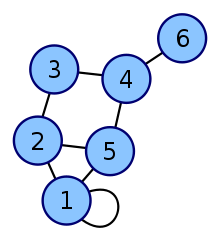
\includegraphics[scale=0.6]{img/graph}
	\caption{Ejemplo de grafo}
	\label{contexto:figura1}
\end{figure}

{\bf Estructura de lista}
\begin{itemize}
	\item {\bf Lista de incidencia:} Las aristas son representadas con un vector de pares (ordenados, si el grafo es dirigido), donde cada par representa una de las aristas.
	\item {\bf Lista de adyacencia:} Cada vértice tiene una lista de vértices los cuales son adyacentes a él. Esto causa redundancia en un grafo no dirigido (ya que A existe en la lista de adyacencia de B y viceversa), pero las búsquedas son más rápidas, al costo de almacenamiento extra. ListAdy=\{ \{1,2,5\}, \{3,5\}, \{4\}, \{5,6\} \}
	\item {\bf Lista de grados:} También llamada secuencia de grados o sucesión gráfica de un grafo no-dirigido es una secuencia de números, que corresponde a los grados de los vértices del grafo.LisGra=(4,3,3,3,2,1).
\end{itemize}

{\bf Estructuras matriciales}
\begin{itemize}
	\item {\bf Matriz de adyacencia:} El grafo está representado por una matriz cuadrada M de tamaño $n^{2}$, donde n es el número de vértices. Si hay una arista entre un vértice x y un vértice y, entonces el elemento m {x, y} es 1, de lo contrario, es 0.
	\begin{figure}[h]
		\centering 
		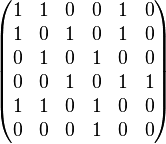
\includegraphics[scale=0.6]{img/matrizadyacencia}
		\caption{Matriz de adyacencia del grafo}
		\label{contexto:figura5}
	\end{figure}
	\item {\bf Matriz de incidencia:} El grafo está representado por una matriz de A. (aristas) por V (vértices), donde [vértice, arista] contiene la información de la arista (1 - conectado, 0 - no conectado).
	\begin{figure}[h]
		\centering 
		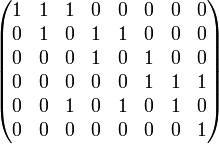
\includegraphics[scale=0.6]{img/matrizincidencia}
		\caption{Matriz de de incidencia del grafo}
		\label{contexto:figura6}
	\end{figure}
\end{itemize}

